\begin{frame}{\tW to \ttbar separation at NLO}
\begin{columns}
\quad
    \begin{column}{0.45\textwidth}
    \begin{block}{\tW decay at NLO}
    \end{block}
    \end{column}
    \quad
    \begin{column}{0.45\textwidth}
    %
    \begin{block}{\ttbar decay}
    \end{block}
    \end{column}
\quad
\end{columns}
    \begin{figure}[htbp]
    \centering
    \begin{subfigure}[b]{0.44\textwidth}
        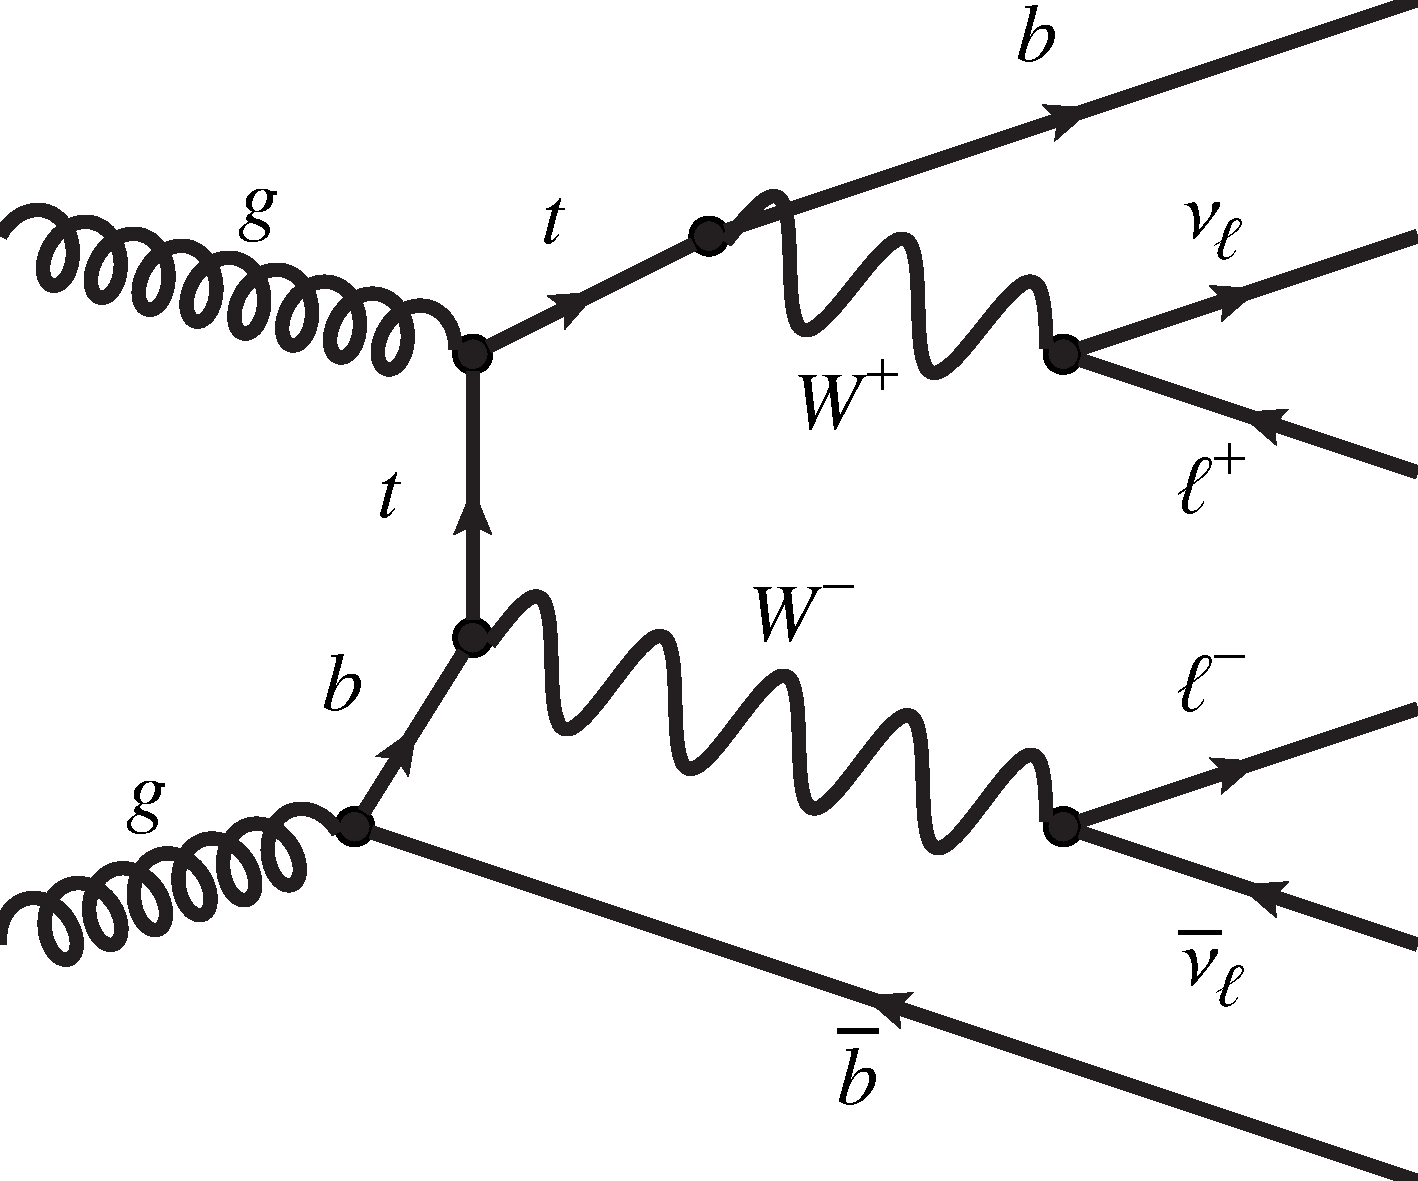
\includegraphics[width=\textwidth]{feynman_diagrams/tw-NLO.pdf}
        %\caption{}
        \label{fig:nlo:ttbar}
    \end{subfigure}
\quad
    \begin{subfigure}[b]{0.44\textwidth}
        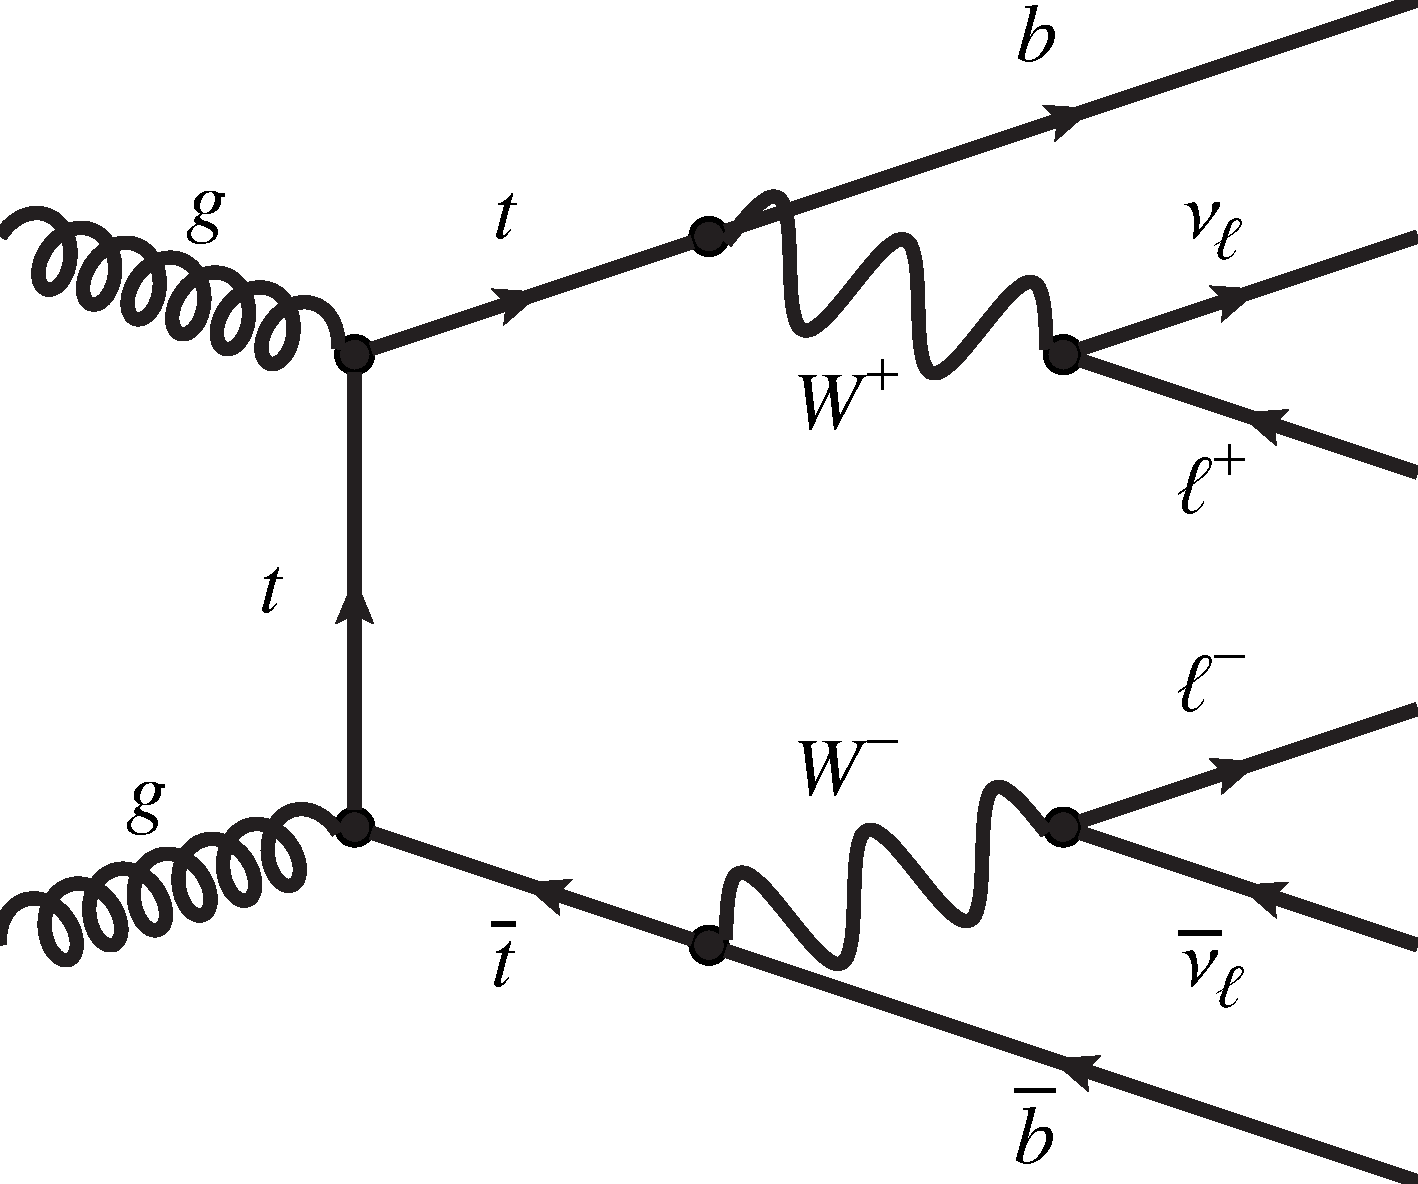
\includegraphics[width=\textwidth]{ttbar-decay}
        %\caption{}
        \label{fig:nlo:tw}
    \end{subfigure}
\end{figure}
%
\begin{columns}
\quad
    \begin{column}{0.45\textwidth}
\begin{itemize}
\item Identical final state
\item Especially problematic in 2j2b region
\end{itemize}
    \end{column}
    \quad
    \begin{column}{0.45\textwidth}
    %
\begin{itemize}
\item Interference at NLO
\item Different Monte Carlo generators
\end{itemize}
    \end{column}
\quad
\end{columns}
\end{frame}

\begin{frame}{Interference in Monte Carlo}
\begin{block}{Amplitude}
\vspace{-0.3cm}
\begin{align*}
|\Aamp|^2 &= |\Atw|^2 + 2 \mathcal{R} \{ \Atw \Att^{\ast} \} + |\Att|^2, \\
&\equiv \Samp + \Iamp + \Damp.
\end{align*}
\end{block}
\begin{block}{Diagram Removal - DR}
\vspace{-0.3cm}
\begin{align*}
| \ADR |^2 = \Samp.
\end{align*}
\end{block}
\begin{block}{Diagram Subtraction - DS}
\vspace{-0.3cm}
\begin{align*}
| \ADS |^2 &= \Samp + \Iamp + \Damp - \widetilde{\Damp},\\
&\approx \Samp + \Iamp.
\end{align*}
\end{block}
\end{frame}

\begin{frame}{Sensitivity to systematic uncertainty}
\vspace{-0.2cm}
\begin{figure}
        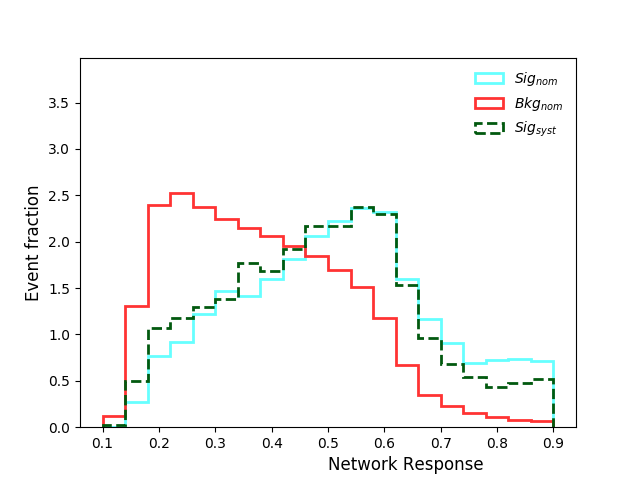
\includegraphics[width=0.8\textwidth]{standard_syst}
%        \caption{Response divided by sample}
%        \label{fig:simple:final:syst}
\end{figure}
\end{frame}

\begin{frame}[c]
\begin{center}
\Huge Adversarial Neural Network
\end{center}
\end{frame}

\begin{frame}{Challenge 2 - Sensitivity to systematic uncertainties}
\begin{block}{Problem 2}
    \begin{itemize}
        \item Minimal sensitivity to the systematic uncertainty
        \item Nominal: $\tW\_DR$, (\ttbar)
        \item Systematic: $\tW\_DS$
    \end{itemize}
\end{block}
\begin{block}{Presented solution}
   \begin{itemize}
       \item Addition of a second classifier for nominal to systematics separation
       \item Bad performance $\longrightarrow$ low sensitivity
   \end{itemize}
\end{block}
\begin{block}{Implementation}
    \begin{itemize}
        \item Feed output into a second net
        \item Iterative training
        \item Combined loss function $\longrightarrow$ Minimax problem
    \end{itemize}
\end{block}
\end{frame}

\begin{frame}{Adversarial neural network}
\vspace{-0.3cm}
    \begin{figure}
        \centering
        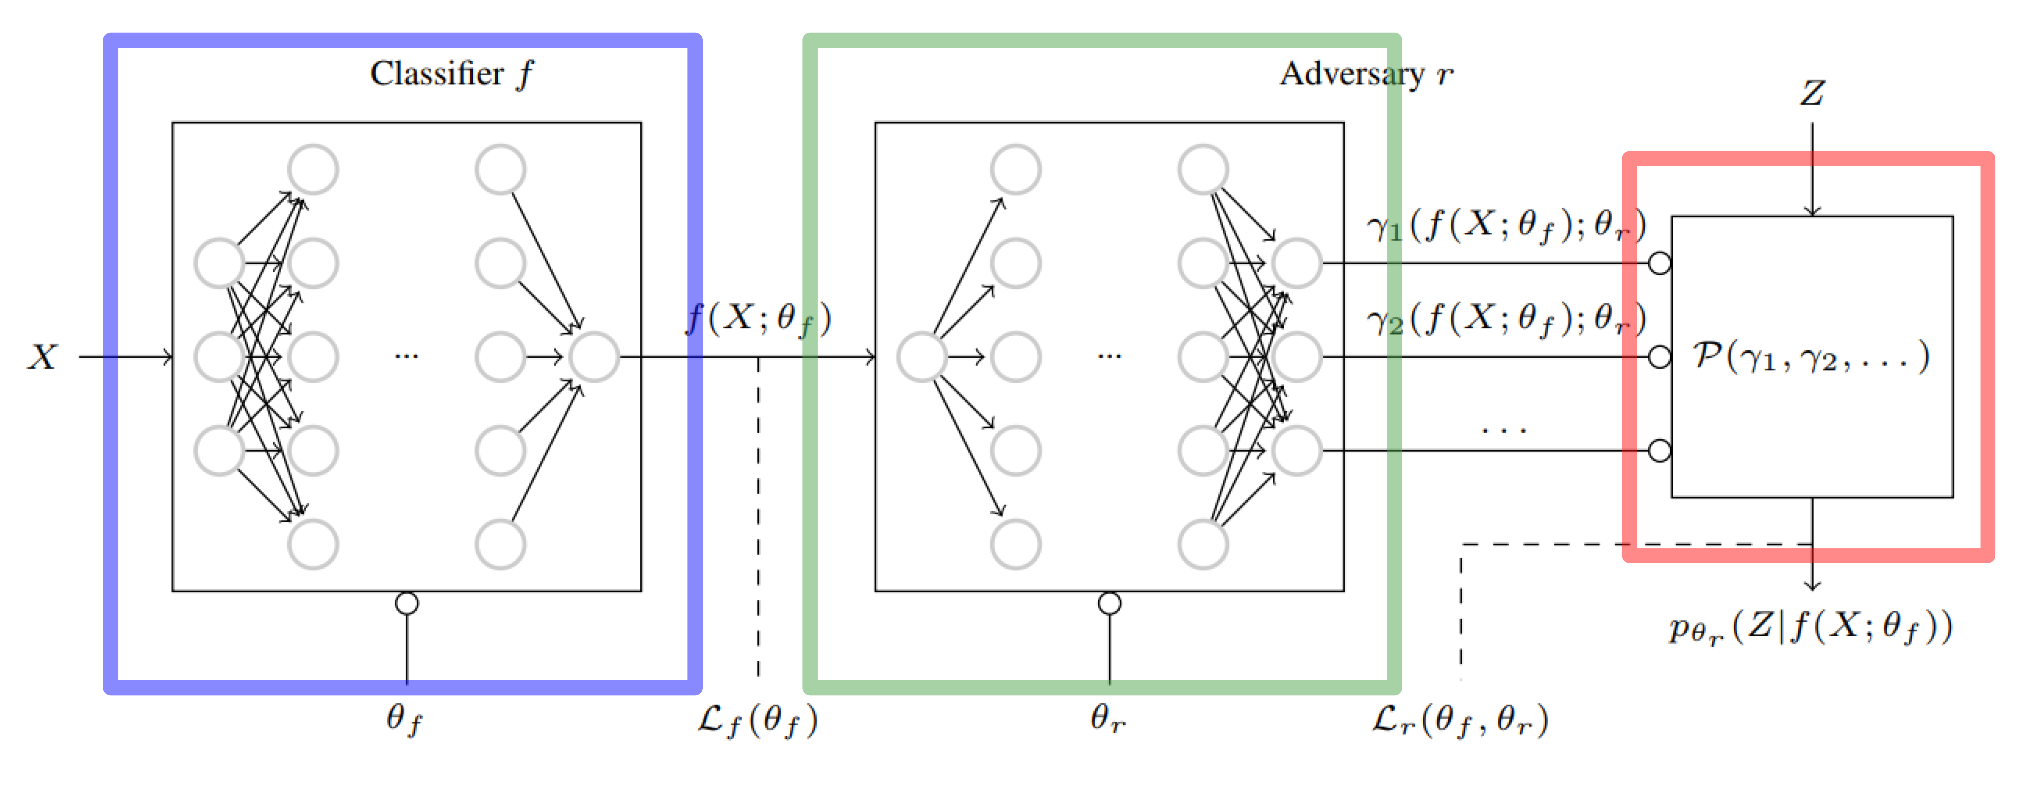
\includegraphics[width=\textwidth]{figures_theory/ANN_paper.eps}
        \caption{(arXiv:1611.01046)}
    \end{figure}
    \begin{equation*}
        \hfsetfillcolor{logo_blue!10}
        \hfsetbordercolor{logo_blue}
        \tikzmarkin{a}(0.3,-0.5)(-0.3,0.55)
        \mathbb{E}(\theta_f, \theta_r) = \mathcal{L}_f(\theta_f) - \lambda \mathcal{L}_r(\theta_f, \theta_r)
        \tikzmarkend{a}
    \end{equation*}
\end{frame}

\begin{frame}{Expected ANN losses}
    \begin{figure}
        \centering
        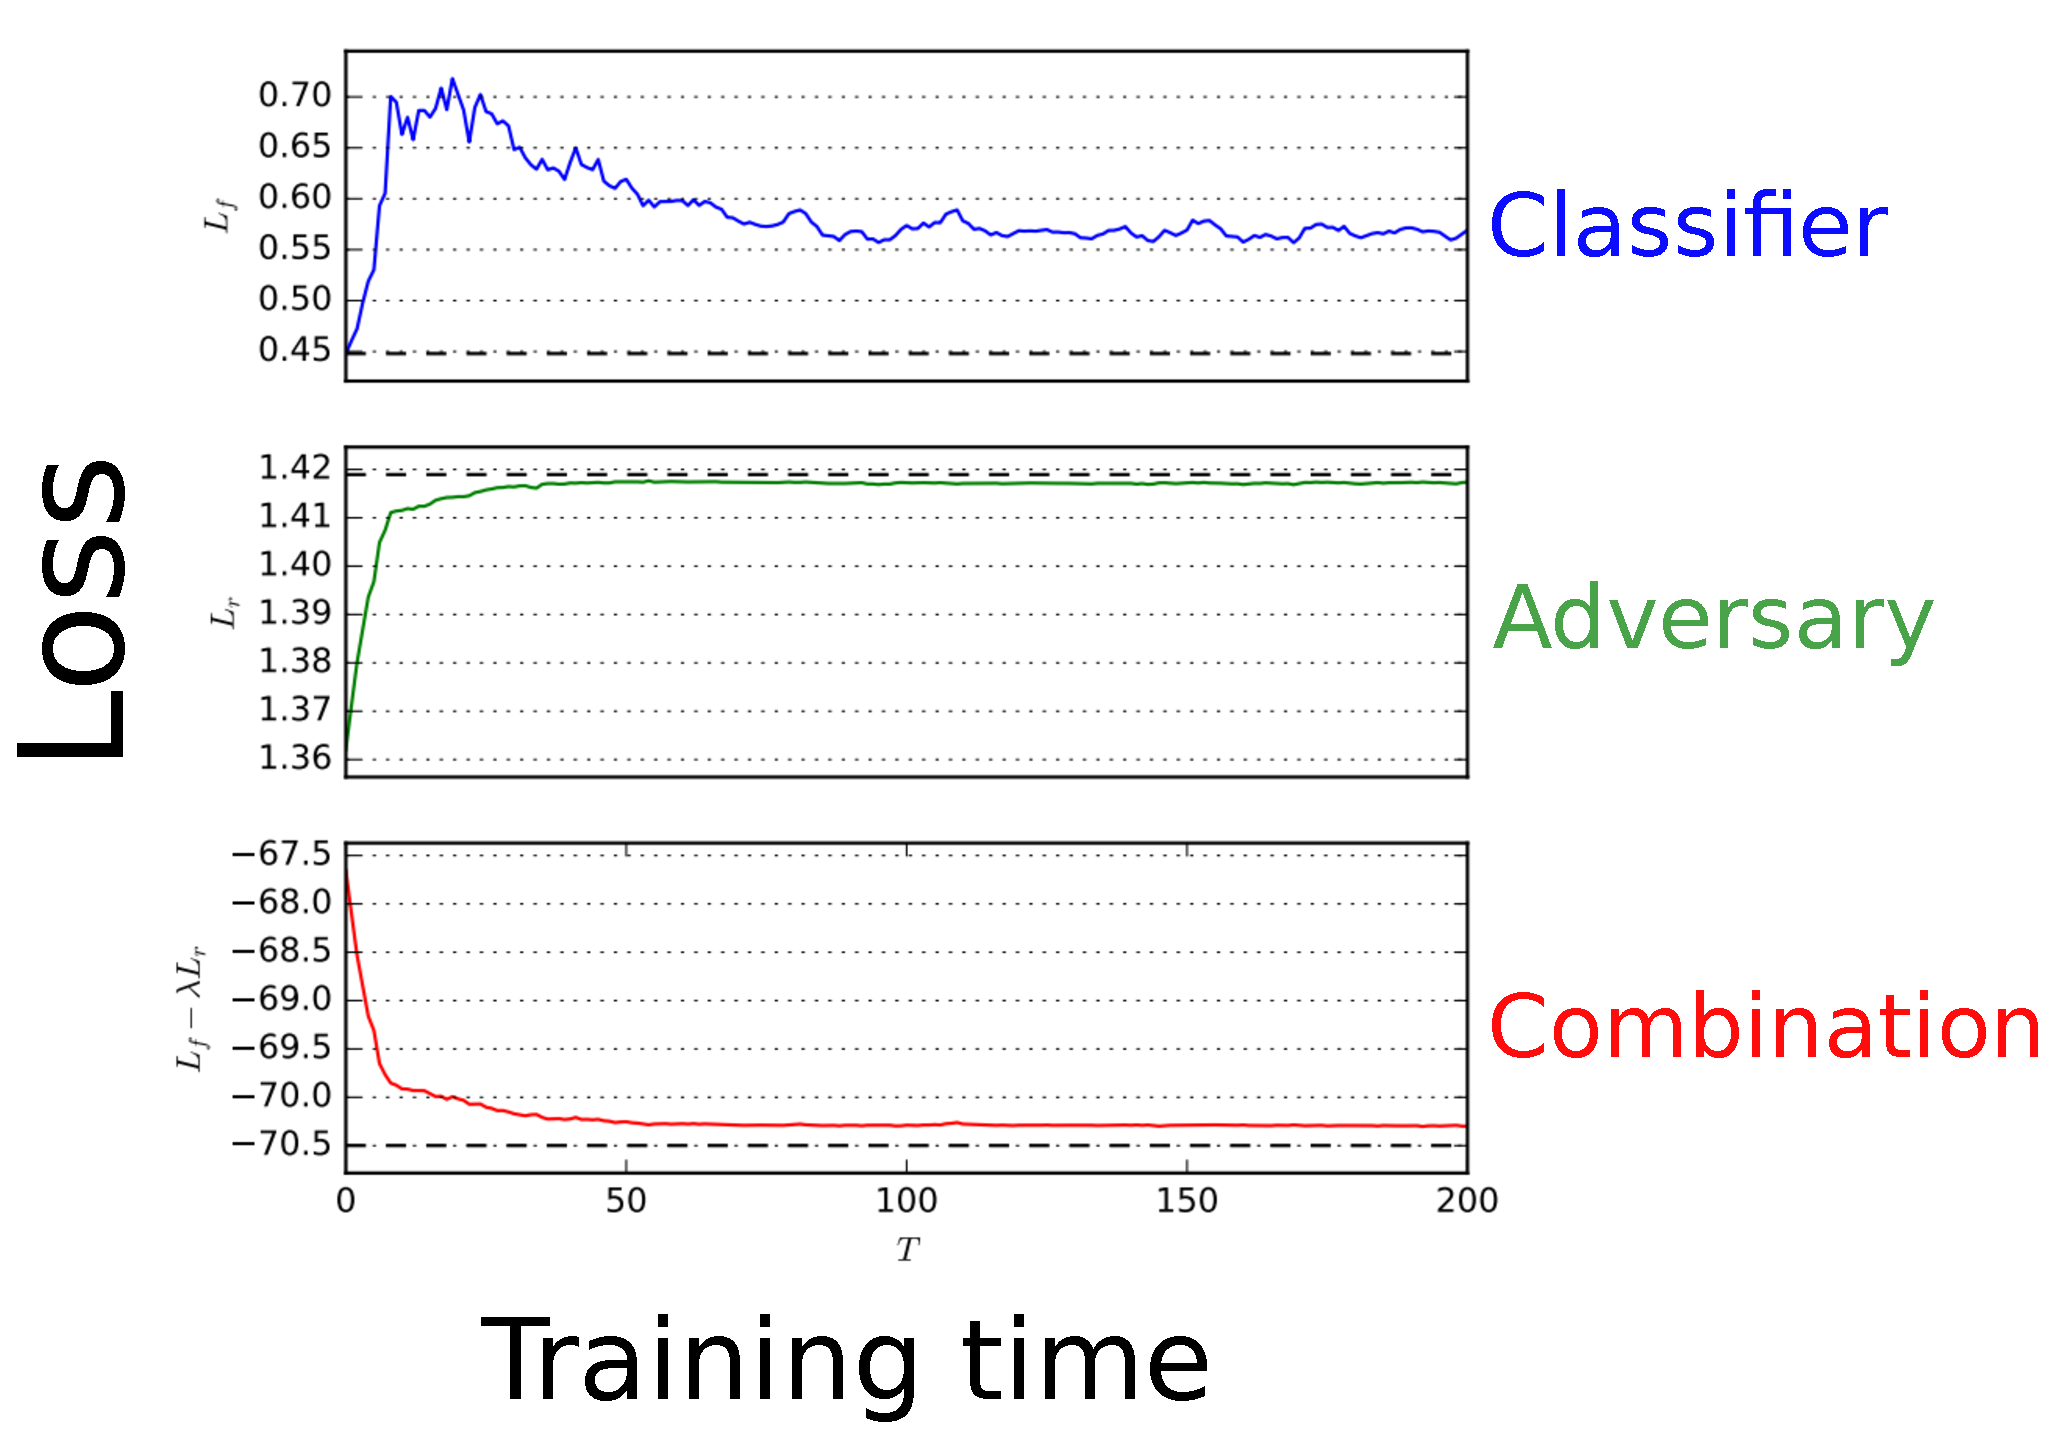
\includegraphics[width=0.9\textwidth]{figures_theory/losses_paper}
        \caption{(arXiv:1611.01046)}
    \end{figure}
\end{frame}